%!TEX root = ../main.tex

\chapter{Preliminaries}\label{sec:prelim}
In this chapter we first give some necessary preliminaries. These background knowledge and notations will then be exploited to introduce our framework, describe our system implementation and present the conducted experiments later in this thesis.

\section{Knowledge Graphs} On the Web, knowledge graphs (KG) are often encoded using the RDF data
model~\cite{rdf}, which represents the content of the graph with a collection of
triples of the form $\tuple{\mi{subject}\;\mi{predicate}\;\mi{object}}$, reflecting positive binary facts (e.g., $\tuple{\mi{bob,livesIn,rome}}$) and unary facts (where $predicate = type$ e.g., $\mi{\tuple{bob,type,scientist}}$) about the world. KGs are naturally treated under the Open World Assumption (OWA), where missing facts are assumed to be unknown rather than false as in the Closed World Assumption (CWA).  %which also known as facts.
% These triples encode
%positive facts about the world, and they are naturally treated under the open world assumption (OWA).

%In this work, we focus on KGs without blank nodes or schema (TBox in the OWL
%terminology). 
%For simplicity, we represent the triples using binary
%predicates. 
We %call this the
%factual representation of the 
consider KG $\cG$ defined over the signature
$\Sigma_{\cG}=\tuple{\mathcal{R}_\cG,\mathcal{C}_\cG}$, where $\mathcal{R}_\cG$ and $\mathcal{C}_\cG$ are sets of
predicates (aka. relations) and constants (aka entities) respectively. 
%E.g., %$\tuple{\mi{alice\;isA\;researcher}}$ in $\cG$ corresponds to $\mi{researcher(alice)}$,  
%$\tuple{\mi{bob \;isMarriedTo\;alice}}$ corresponds to $\mi{isMarriedTo(bob,alice)}$ in the factual representation. 
Relying on \cite{DBLP:conf/semweb/DarariNPR13} we define the gap between the ideal graph %The ideal graph 
$\cG^i$ (a graph containing all possible correct facts with constant and relation from $\Sigma_{\cG}$) and the available graph $\cG$. 
%Thus, we define the incomplete actual graph $\cG$ as 

\begin{definition}[Incomplete data source] An incomplete data source is a pair
    $G = (\cG, \cG^i)$ of two KGs, where $\cG\subseteq \cG^i$ and
    $\Sigma_{\cG}=\Sigma_{\cG^i}$. 
\end{definition}

\section{Non-monotonic Logic Programs}
\label{sec:non-prog}
In this work, we rely on the standard definitions of logic programs \cite{DBLP:books/sp/Lloyd87}.
%logic program in the standard way~\cite{DBLP:books/sp/Lloyd87}. 
In short, a \emph{(non-monotonic) logic program} $P$ is a set of rules $r$ of the form:
\begin{equation}
H\leftarrow B, \naf E
\end{equation}
\noindent where $H$ is a standard first-order atom of the form $a(\vec{X})$ known as the rule head and denoted as $\mi{head(r)}$; $B, \naf E$ is the rule body and denoted as $body(r)$, in which $B$ is a conjunction of positive atoms of the form $b_1(\vec{Y_1}),\dotsc,b_k(\vec{Y_k})$ to which we refer as $\mi{body^+(r)}$. Moreover, $\naf E$, to which we refer as $\mi{body^-(r)}$, with slight abuse of notation, denotes the conjunction of atoms $\naf\, b_{k+1}(\vec{Y_{k+1}}),\dotsc,\naf\, b_n(\vec{Y_{n}})$, where $\naf$ is called \emph{negation as failure (NAF)} or \emph{default negation}.
Here, $\vec{X},\vec{Y_1},\ldots,\vec{Y_{n}}$ are tuples of either constants or
variables whose length corresponds to the arity of the predicates
$a,b_1,\ldots,b_n$ respectively. Moreover, the rule $r$ is called Horn, if all head variables appear in the body, and the negated part $E$ is empty. The signature of $P$ is given as $\Sigma_{\mi{P}}=\tuple{\mathbf{P},\mathbf{C}}$, where $\mathbf{P}$ and $\mathbf{C}$ are sets of predicates and constants occurring in $P$ respectively.  %Positive, negative body and head of a rule $r$ are defined as usual \cite{DBLP:books/sp/Lloyd87} and denoted resp. as $B^+(r),B^-(r)$ and $H(r)$.

We consider answer set semantics \cite{GL1988} in this work. A logic program P is called \textit{ground} if no variable appear in any rule $r$ of $P$. A ground instantiation $Gr(P)$ of a non-ground logic program $P$ is obtained by replacing its variables by constants of $\mathbf{C}$ in all
possible ways. The \textit{Herbrand Universe} $HU(P)$ of a program $P$ is the set of all constants appearing in P. The \textit{Herbrand Base} $HB(P)$ is the set of all possible ground atoms created from predicates in $\mathbf{P}$ and constants in $\mathbf{C}$. An \textit{Herbrand Interpretation} of $P$ is any subset of $HB(P)$. An interpretation $I$ is a \textit{Model} of a program $P$ iff it satisfies every rule $r$ of $P$, i.e., for every substitution  of variables of $r$ with constants in $\mathbf{C}$, if $I \models body(r)$ then we also have $I \models head(r)$. A model $I$ is called minimal if there does not exist any model $I' \subset I$. The set of all subset-inclusion minimal models of $P$ is denoted by $MM(P)$.

An interpretation $I$ of $P$ called an \textit{Answer Set} (or \textit{Stable Model}) of $P$ iff  $I \in MM(P^I)$, where $P^I$ is the Gelfond-Lifschitz (GL) reduct of $P$ constructed from $Gr(P)$ by excluding 
(i) any rule $r$ that $I \not\models body^-(r)$ and (ii) negated part from the remaining rules. The set consisting of all answer sets of $P$ is denoted as $AS(P)$.
\begin{example}
Consider the following logic program $P$:
\begin{align*}
P = \left\{
           \begin{array}{@{\,}l@{~~}l@{}}
              \mbox{(1) }worksFor(Alice, ITech);\;
              \mbox{(2) }hasHeadquartersIn(ITech,Paris);\\
              \mbox{(3) }livesIn(X,Y) \leftarrow worksFor(X,Z), hasHeadquartersIn(Z,Y),\\
              \hspace{18em}\naf locatedIn(Y,USA);
            \end{array}
            \right\}
\end{align*}
We achieve $Gr(P)$ by replacing $X,Y,Z$ by $Alice, Paris, ITech$, correspondingly. With $I = \{worksFor(Alice, ITech), hasHeadquartersIn(ITech,Paris), livesIn(Alice, Paris)\}$, the Gelfond-Lifschitz reduct $P^I$ consists of facts (1), (2) and the rule $livesIn(Alice,Paris) \leftarrow worksFor(Alice,ITech), hasHeadquartersIn(ITech,Paris)$. Because $I$ is a minimal model of $P^I$, we conclude that $I$ is also an answer set of $P$.\qed
\end{example}

%\begin{figure}[t]
%\centering
%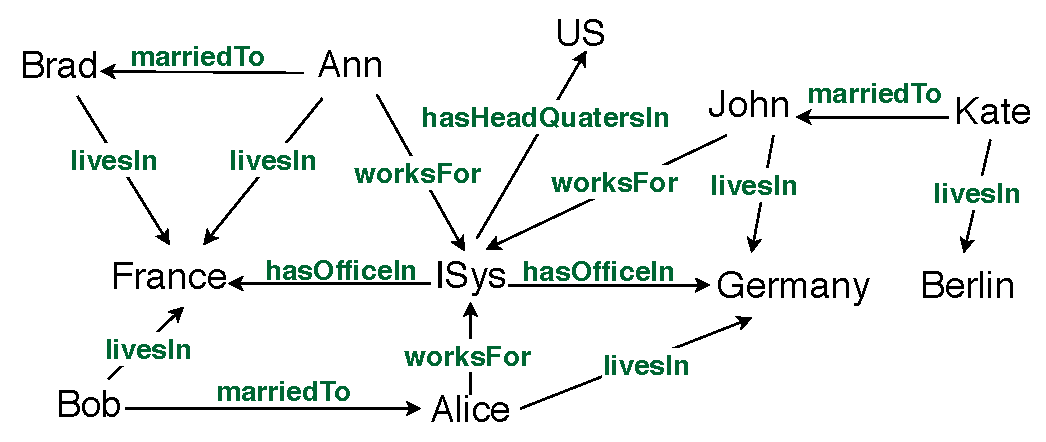
\includegraphics[width=0.8\textwidth]{figures/kg3.pdf}
%%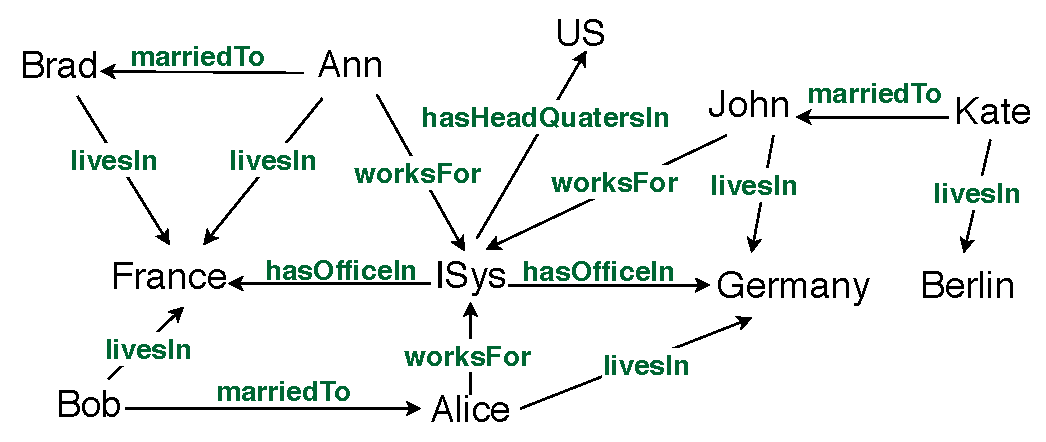
\includegraphics[scale=0.32]{figures/kg3.pdf}
%\caption{An example of a knowledge graph.}
%\label{fig:kg}
%\end{figure}

\section{Relational Association Rule Learning}
Association rule learning concerns the discovery of frequent patterns in a data set and the subsequent transformation of these patterns into rules.
A \emph{conjunctive query} over $\cG$ is of the form $Q(\vec{X}) \text{ :- } p_1(\vec{X_1}),\dotsc,p_m(\vec{X_m})$, where $\vec{X_i}$ are binary or unary vectors of variables and/or constants. Its  right-hand side (i.e., body) is a finite set of atomic formulas over $\Sigma_{\cG}$, while the left-hand side (i.e., head) is a tuple of variables occurring in the body and/or constants. The \emph{answer} of $Q$ on $\cG$ is the set $Q(\cG) = \{ \nu(\vec{X}) \mid \nu \text{ is a function from variables to } \mathcal{C} \text{ and } \forall i: p_i(\nu(\vec{X_i})) \in \cG \}$.
%As in \cite{DBLP:conf/ilp/DehaspeR97}, t
The \emph{support} of
$Q$ in $\cG$ is the number of distinct tuples in the answer of $Q$ on $\cG$. 
\begin{example}
\label{ex:ass_query_support}
The support of the following query:
\[Q(X,Y,Z) \text{ :- } worksFor(X,Y), hasOfficeIn(Y,Z)\]
over the KG $\cG$ in Fig. \ref{fig:kg} asking for people, their companies and the companies' locations is 12. \qed
\end{example}
An \emph{association rule} is of the form $Q_1 \Rightarrow  Q_2$, such that $Q_1$ and $Q_2$ are both conjunctive queries and $Q_1 \subseteq Q_2$, i.e., $Q_1(\cG')\subseteq Q_2(\cG')$ for any possible KG $\cG'$. In this work we exploit association rules for reasoning purposes, and thus (with some abuse of notation) treat them as logical rules, i.e., for $Q_1\Rightarrow Q_2$ we write $Q_2\backslash Q_1 \leftarrow Q_1$, where $Q_2 \backslash Q_1$ refers to the set difference between $Q_2$ and $Q_1$ seen as sets of atoms.
\begin{example}
Consider the query $Q$ from Example \ref{ex:ass_query_support} and also the following query:
\[Q'(X,Y,Z) \text{ :- } worksFor(X,Y), hasOfficeIn(Y,Z), livesIn(X,Z)\]
the \textit{association rule} $Q \Rightarrow Q'$ can be written as the following logical rule:\[livesIn(X,Z) \leftarrow worksFor(X,Y), hasOfficeIn(Y,Z)\]\qed
\end{example}

\begin{figure}[t]
\centering
\begin{tikzpicture}[->,>=stealth',auto,node distance=3cm,
  thick,main node/.style={font=\bfseries}]

  \node[main node] (1) {Brad};
  \node[main node] (2) [right=3cm of 1] {Ann};
  \node[main node] (3) [right=7.5cm of 1] {US};
  \node[main node] (5) [right=11cm of 1] {Kate};  
  \node[main node] (6) [below right =1.5cm and 0.75cm of 1] {France};
  \node[main node] (4) [right=7cm of 6] {John};  
  \node[main node] (7) [right=3cm of 6] {ISys};

  \node[main node] (10) [below left=1.5cm and 1cm of 6] {Bob};  
    \node[main node] (9) [right=11cm of 10] {Berlin};  
  \node[main node] (11) [right=3cm of 10] {Alice};  
  \node[main node] (8) [right=3cm of 11] {Germany};  
  
  \path[every node/.style={color=teal,fill=white,font=\small}]
    (2) edge node [right=-23pt] {\textit{marriedTo}} (1)
    (5) edge node [right=-30pt] {\textit{marriedTo}} (4)
    (10) edge node [right=-27pt] {\textit{marriedTo}} (11)    
    (1) edge node [right=-20pt] {\textit{livesIn}} (6)
    (2) edge node [right=-20pt] {\textit{livesIn}} (6)
    (5) edge node [right=-20pt] {\textit{livesIn}} (9)
    (4) edge node [right=-20pt] {\textit{livesIn}} (8)
    (11) edge node [right=-20pt] {\textit{livesIn}} (8)
    (10) edge node [right=-20pt] {\textit{livesIn}} (6)
    (2) edge node [right=-23pt] {\textit{worksFor}} (7)
    (4) edge node [right=-23pt] {\textit{worksFor}} (7)
    (11) edge node [right=-25pt] {\textit{worksFor}} (7)
    (7) edge node [right=-23pt] {\textit{hasOfficeIn}} (6)
    (7) edge node [right=-25pt] {\textit{hasOfficeIn}} (8)
    (7) edge node [right=-38pt] {\textit{hasHeadQuatersIn}} (3);
\end{tikzpicture}
\caption{An example knowledge graph.}
\label{fig:kg}
\end{figure}

\subsection{Rule Types}
Below we recap various rule types.
\begin{definition}[Connected rule] A rule is \textit{connected} if any two of its variables are connected through a series of atoms, where two atoms are connected if they share a variable or constant.
\end{definition}
\begin{example}
The rule below is connected:
\[isMusician(X) \leftarrow playsForBand(X, Y)\]
because variables X and Y are connected through the atom $playsForBand(X, Y)$. In contrast, the following rule is \textbf{not} connected:
\[speaks(X, English) \leftarrow livesIn(X, UK), worksIn(Y, US)\]
This rule seems to be meaningless, since there is no connection between $X$ and $Y$. If we remove the last atom $worksIn(Y, US)$, then the rule becomes connected. 
\qed
\end{example}
\begin{definition}[Closed rule] A \textit{closed} rule is a connected rule, whose every variable appears at least twice.
\end{definition}
\begin{example}
Rules $r_1$ and $r_2$ from Equations \ref{eq:ex-rule-1} and \ref{eq:ex-rule-2} are closed. An example of a non-closed rule is: \[musician(X) \leftarrow playsInstrument(X, Y)\]\qed
\end{example}

\begin{definition}[Recursive rule] A rule is called \textit{recursive} if its body contains the head predicate, since. Applying a recursive rule on the knowledge graph many times might predict new more facts.
\begin{example}
The rule $r_2$ is a recursive rule. In contrast, $r_1$ is \textbf{not} recursive, because the head predicate "livesIn" does not appear in the rule body. \qed
\end{example}

\end{definition}
\begin{definition}[Safe rule] A rule is \textit{safe} if every variable in its negated part appears in the positive part of the rule. %In other words, a rule is safe iff it is \textit{connected} and its Horn part is \textit{closed}.
\end{definition}
\begin{example}
The rule $r_3$ in Equation \ref{eq:ex-rule-3} is $safe$. In contrast, the following rule is unsafe:\[livesIn(Y,Z) \leftarrow marriedTo(X,Y), livesIn(X,Z), \naf doResearchAt(Y,T)\]
because variable T does not appear in the positive part of the rule.\qed
\end{example}
\subsection{Rule Statistics}
To quantify the quality of association rules on the knowledge graph, various rule metrics have been proposed. We list some prominent metrics below. Given a KG $\cG$, a rule $r : H \leftarrow B, \naf E$, where $H = h(X,Y)$ and $B,E$ involve variables from $\vec{Z}\supseteq \{X,Y\}$, the following measures can be computed:\\
- \textbf{Rule support} (or \textit{support}): indicates the absolute number of instantiations of a rule that are true in the knowledge graph.
\begin{equation}\label{eq:supp}
\textit{supp}(r,\cG) = \#(X,Y): H \in \cG, \exists \vec{Z}:B\in \cG,E \not \in \cG\\
\end{equation}
where $\# \beta : \mathcal{B}$ denotes the number of $\beta$ that fulfill the condition $\mathcal{B}$.\\
- \textbf{Body support}: indicates the absolute number of instantiations of rule's body in the knowledge graph.
\begin{equation}\label{eq:body_supp}
\textit{b-supp}(r,\cG) = \#(X,Y):\exists \vec{Z}:B\in \cG, E \not \in \cG
\end{equation}
- \textbf{Head support}: indicates the absolute number of instantiations of rule's head in the knowledge graph. In other words, this is the total number of facts in the KG over the head predicate $h$.
\begin{equation}\label{eq:head_supp}
\textit{h-supp}(r,\cG) = \#(X,Y): H \in \cG
\end{equation}
\begin{example}
Consider the two rules $r_1$, $r_2$ from Equations~\ref{eq:ex-rule-1} and \ref{eq:ex-rule-2} and the KG $\cG$ from Fig. \ref{fig:kg}. For the rule $r_1$, we have $supp(r_1,\cG)=3$ and $\textit{b-supp}(r_1,\cG) = 6$. Similarly, for $r_2$, we have $supp(r_2,\cG)=1$ and $\textit{b-supp}(r_2,\cG) = 3$. Moreover, $\textit{h-supp}(r_1,\cG) = \textit{h-supp}(r_2,\cG) = 6$, since there are totally 6 facts in $\cG$ with the head predicate $"livesIn"$.
\qed
\end{example}
\noindent- \textbf{Head coverage}: While support gives us the absolute number of correct rule instantiations, it does not tell us how much the rule affects the knowledge graph, since it does not take into account the size of the knowledge graph. Head coverage fixes this issue by reflecting the ratio of the rule support to the head support.
\begin{equation}\label{eq:hc}
\textit{hc}(r,\cG) = \frac{supp(r,\cG)}{\textit{h-supp}(r,\cG)}
\end{equation}
\begin{example}
We have $hc(r_1,\cG) = \frac{3}{6}$ and $hc(r_2,\cG) = \frac{1}{6}$.
\qed
\end{example}

\noindent- \textbf{Standard Confidence} (or \textit{confidence}): treats the knowledge graph under the Closed World Assumption (CWA). The standard confidence returns a number between $[0,1]$, which corresponds to the ratio of the rule support to the body support. Formally:
\begin{equation}\label{ex:m}
\mi{conf}(r,\cG) = \frac{\mi{supp}(r,\cG)}{\textit{b-supp}(r,\cG)}
\end{equation}
\begin{example}
We have $conf(r_1,\cG) = \frac{3}{6}$ and $conf(r_2,\cG) = \frac{1}{3}$. Moreover, for the following rule with negation:
\[\mi{r_4:\,livesIn(Y,Z) \leftarrow marriedTo(X,Y), livesIn(X,Z), not\;researcher(X)}\]
states that married people live together unless one is a researcher, 
and $\cG'=\cG\cup\{\mi{researcher(Bob)}\}$, we have $\mi{conf(r_4,\cG') = \frac{1}{2}}$.\qed
\end{example}
\noindent- \textbf{PCA Confidence} \cite{amie}: is based on the Partial Closed-world Assumption (PCA), which assumes that the data of the knowledge graph is added in batches. More specifically, for each subject $s$ and relation $p$, if there exists some object $o'$ such that $p(s,o') \in \cG$, then all possible true triples $p(s,o)$ are assumed to be presented in $\cG$. The \textit{PCA confidence} is defined as follows:
\begin{equation}\label{eq:pca_conf}
\mi{conf_{pca}}(r, \cG) = \frac{\textit{supp}(r, \cG)}{\#(X,Y): \exists \vec{Z}: B \in \cG, E \notin \cG  \wedge \exists Y': h(X,Y')\in \cG}
\end{equation}
Similar to the \textit{standard confidence}, the \textit{PCA confidence} also gives us a value between $[0,1]$.
\begin{example}
We have $conf_{pca}(r_1,\cG) = \frac{3}{6}$, $conf_{pca}(r_2,\cG) = \frac{1}{3}$ and $conf_{pca}(r_4,\cG') = \frac{1}{2}$. If Alice was not known to live in Germany in $\cG$, then $\mi{conf_{pca}(r_2,\cG)}=\frac{1}{2}$. \qed
\end{example}

\noindent- \textbf{Conviction} \cite{trantowards}: is shown to correlate with the rule predictive power \cite{Azevedo2007}.
%by measuring the intensity of rule's implication \cite{DBLP:conf/eurogp/MinhdNT18}
\textit{Conviction} is defined as follows:
\begin{equation}\label{eq:conv}
\textit{conv}(r,\cG) = \frac{1 - \textit{rel-supp}(h, \cG)}{1-\textit{conf}(r,\cG)}
\end{equation}
where $\textit{rel-supp}(h)$ is the relative support of the head, which is measured by:
\begin{equation}
\textit{rel-supp}(h, \cG) = \frac{\textit{h-supp}(r,\cG)}{(\# X: \exists Y' :h(X,Y') \in \cG) \times (\#Y :\exists X': h(X',Y) \in \cG)}
\end{equation}
\begin{example}
We have $\textit{rel-supp}(livesIn, \cG) = \frac{6}{6 \times 3} = \frac{1}{3}$. Thus, $conv(r_1,\cG) = \frac{1 - \frac{1}{3}}{1 - \frac{3}{6}} = \frac{4}{3}$ and $conv(r_2,\cG) = \frac{1 - \frac{1}{3}}{1 - \frac{1}{3}} = 1$.
\qed
\end{example}
Unlike standard confidence and PCA confidence, conviction gives us a value in $[0,\infty]$.
\subsection{Rule-based KG Completion}

Given a rule $r$ and a KG $\cG$ the application of $r$ on $\cG$ results in a rule-based graph completion defined relying on the answer set semantics as recapped in Section \ref{sec:non-prog}.

\begin{definition}[Rule-based KG completion]\label{def:graphcompl}
Let $\cG$ be a KG over the signature $\Sigma_{\cG}=\tuple{\mathbf{R},\cC}$ and let $r$ be a rule %$r$ be a set of rules 
mined from $\cG$, i.e. a rule over $\Sigma_{\cG}$.
Then the \emph{completion of $\cG$} using $r$ is a graph $\cG_{r}$ constructed from any answer set of $r \cup \cG$. 
\end{definition}

\begin{example}
The application of $r_1$ and $r_2$ on $\cG$ from Figure \ref{fig:kg} results respectively in:\\
\textit{ - $\cG_{r_1} = \cG\;\cup$ \{livesIn(Ann,Germany), livesIn(John,France), livesIn(Alice,France)\}}\\
\textit{ - $\cG_{r_2} = \cG\;\cup$ \{livesIn(Alice,France), livesIn(John, Berlin)\}}. \qed
\end{example}

Note that $\cG^i$ is the perfect completion of $\cG$, i.e., it is supposed to contain all
correct facts with entities and relations from $\Sigma_{\cG}$ that hold
in the current state of the world. The goal of the rule-based KG completion is to extract from $\cG$ a set of rules $\cR$ such that $\cG_{\cR} = \cup_{r\in \cR}\cG_{r}$ is as close to $ \cG^i$ as possible.

\section{Link Prediction Embedding Models} 
Recently a vast amount of latent-based approaches for statistical relational learning have been proposed  (see \cite{Nickel0TG16} for overview), which address the KG completion problem by reducing it to a representation learning task, where the main goal is to represent entities and relations of $\cG$ in a
low-dimensional, say $d$-dimensional, vector (aka embedding) and relying on these representation estimate the likelihood (not necessary probability) of the potentially missing facts. 
%vector space $\vec{h}, \vec{t}, \vec{r} \in I\!R^d$ such that for $\tuple{h,r,r}\in \cG$ it holds that $\vec{h}+\vec{r}\approx \vec{t}$.  
Some models rely exclusively on the triples in the available graph and estimate the likelihood of the missing ones~\cite{Bordes:NIPS2013,DBLP:conf/aaai/NickelRP16}, while others may utilize external resources (\eg text)~\cite{DBLP:conf/aaai/0005HMZ17}. 

%For a pair $\tuple{\cG, \cE}$, $\cE$ is an embedding model of $\cG$, if for each triple $\tuple{s,p,o}\in \cG$, there exists a vector $v \in \cE$. 
Typical embedding models define a scoring function $\xi: \cR_\cG \times \cC_\cG \times \cC_\cG \rightarrow \mathbb{R}$ that given an $\tuple{\mi{s,p,o}}$ triple computes a numerical value reflecting its likelihood. The higher score is, the more plausible the triple is. While in this work we experiment with several selected KG embedding models, our general rule learning approach can conceptually exploit any model. Some prominent embedding models have been recapped in related work of Chapter \ref{sec:related-work}.

%If we treat a KG embedding model as an oracle, then the questions that one can pose to it include $\tuple{s,p,o}$, $\tuple{s,p,?}$, $\tuple{?,p,o}$ and $\tuple{s,?,o}$. Apart from asking for the plausibility score of an individual fact $\tuple{s,p,o}$, the existing embedding models can also output a list of ordered potentially missing objects given a $\tuple{s,p,?}$ by ranking them based on the plausibility score. Other two types of queries that can be posed to an embedding model including $\tuple{?,p,o}$ and $\tuple{s,?,o}$ could be treated similarly.


